\documentclass{beamer}

\usetheme{Malmoe}

\setbeamertemplate{subsection in toc}[circle]
\setbeamertemplate{section in toc}[circle]

%\addtobeamertemplate{footline}{\insertframenumber/\inserttotalframenumber}

\newcommand*\oldmacro{}%
\let\oldmacro\insertshorttitle%
\renewcommand*\insertshorttitle{%
  \oldmacro\hfill%
  \insertframenumber\,/\,\inserttotalframenumber}

\AtBeginSection[] {
\begin{frame}\frametitle{Table of contents}

  \begin{columns}[t]
  \begin{column}{6cm}
  \tableofcontents[sections={1-2},currentsection,hideothersubsection]
  \end{column}
  \begin{column}{5cm}
  \tableofcontents[sections={3-5},currentsection,hideothersubsection]
  \end{column}
  \end{columns}

\end{frame}
}

\begin{document}
\subtitle{Internship Presentation}

\title{Design \& certification process\\ of the Mission M108}

\author{Melanie Bombardiere}

\date{January 21st, 2014}

\begin{frame}
  \titlepage
\end{frame}

\section{Introduction}

\subsection{Lambert Aircraft Engineering}

\begin{frame}\frametitle{Lambert Aircraft Engineering -- Presentation}
\begin{figure}[ht!]
	\begin{center}
		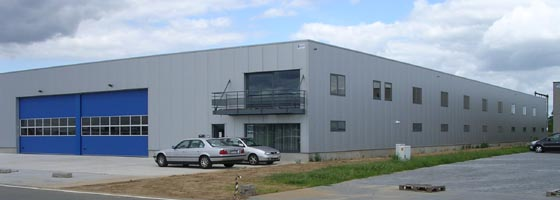
\includegraphics[width=10cm]{pics/PIC001.jpg}
		\label{fig:LAE}
	\end{center}
\end{figure}

\begin{itemize}
    \item limited series production of aircraft;
    \item avionics maintenance.
  \end{itemize}
\end{frame}

\subsection{The Mission M108 LSA}

\begin{frame}\frametitle{The Mission M108 LSA -- Presentation}

\begin{figure}[ht!]
	\begin{center}
		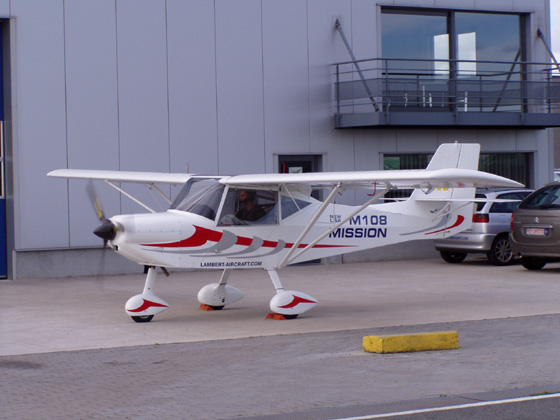
\includegraphics[width=10cm, trim = 0cm 1.5cm 0cm 2cm,clip]{pics/M108BIS.JPG}
		\label{fig:M108}
	\end{center}
\end{figure}

  \begin{itemize}
    \item two seater single engine light sport aircraft;
    \item welded tubular structure;
    \item Rotax 912iS engine.
  \end{itemize}
\end{frame}

\begin{frame}\frametitle{The Mission M108 LSA -- Presentation}
  \begin{itemize}
    \item ASTM: American Society for Testing and Materials;\\
Light Sport Aircraft characteristics:
\begin{itemize}
\item maximal weight: 600kg
\item Single engine
\item Maximum 2 seats
\item ...
\end{itemize}
    \item FAA: Federal Aviation Administration;
    \item EASA: European Agency for Safety Aviation.
  \end{itemize}
\end{frame}

\section{CAD and design work}

\begin{frame}
\begin{figure}[ht!]
	\begin{center}
		\includegraphics<1>[width=10cm,trim = 3cm 3cm 3cm 3cm, clip]{pics/M108-3D.pdf}
		\includegraphics<2>[width=7.5cm,trim = 8cm 4cm 15cm 11cm, clip]{pics/M108-3D.pdf}
		\caption{The Mission M108}
		\label{fig:M1083D}
	\end{center}
\end{figure}
\end{frame}

%\subsection{Radiator}

%\begin{frame}\frametitle{Radiator}
%\begin{figure}[ht!]
%	\begin{center}
%		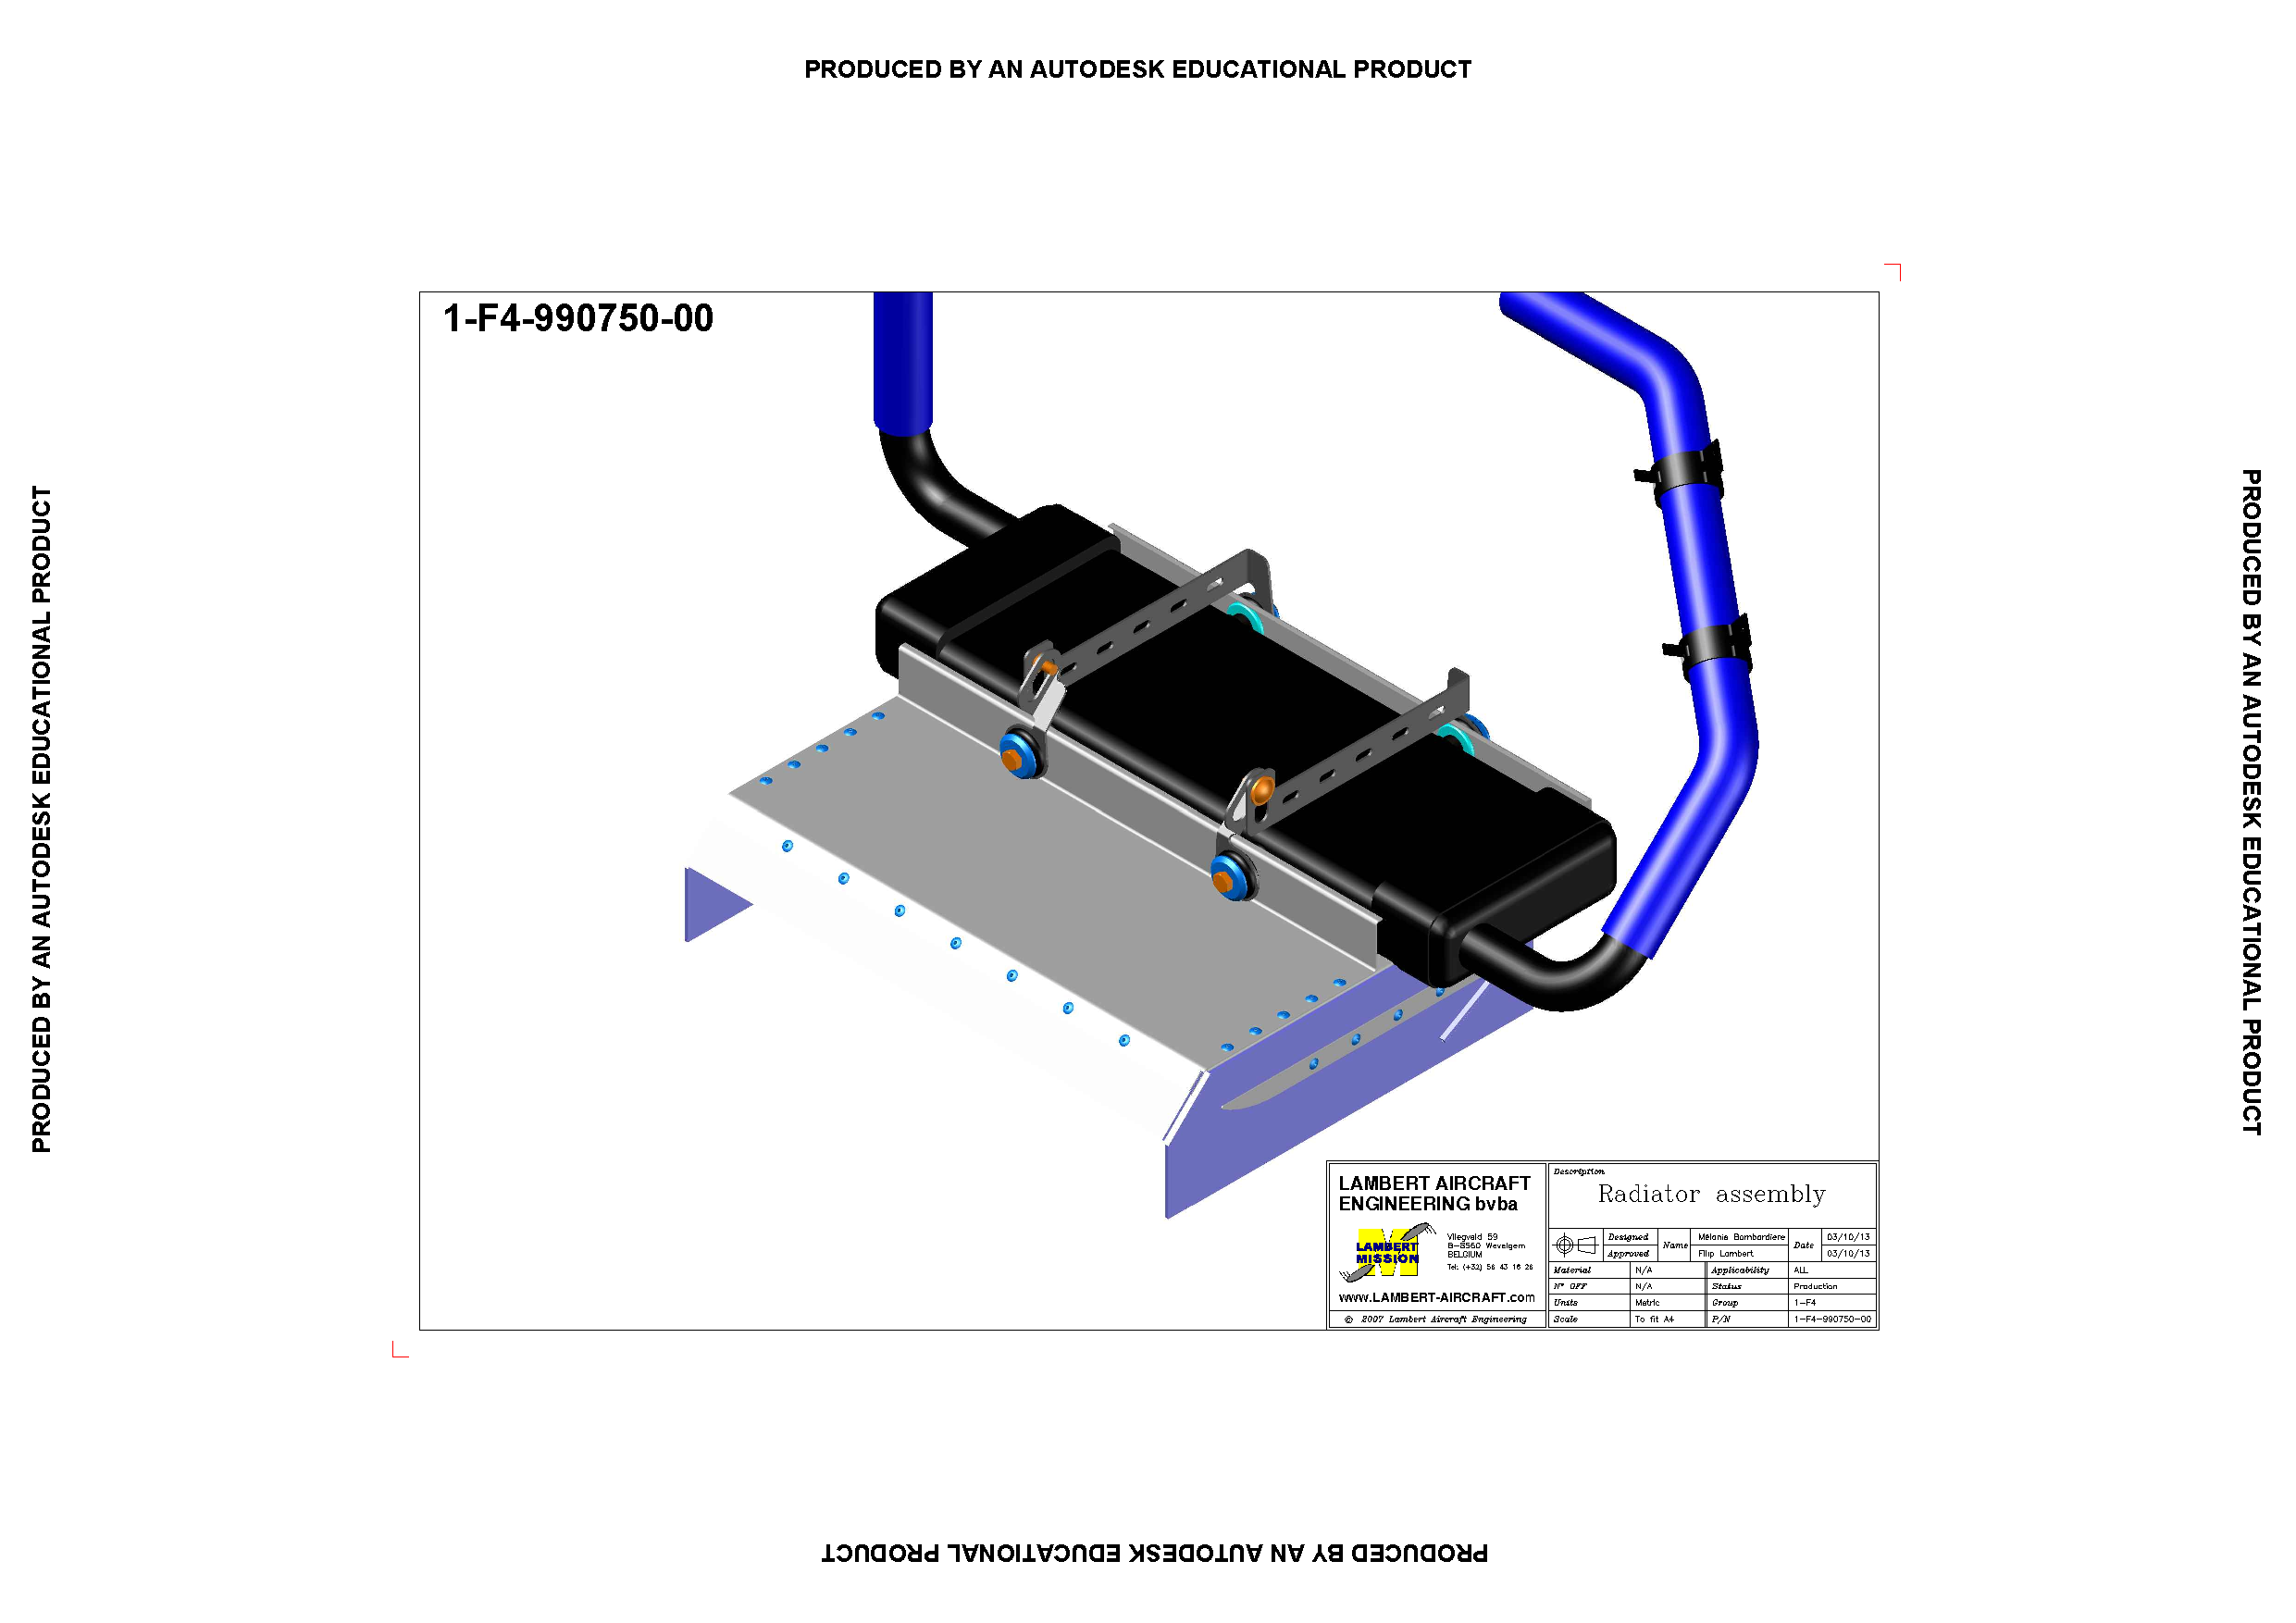
\includegraphics[width=7.5cm,trim = 5cm 5cm 5cm 5cm, clip]{pics/PIC008.pdf}
%		\caption{The radiator assembly}
%		\label{fig:PIC008}
%	\end{center}
%\end{figure}
%\end{frame}

%\begin{frame}\frametitle{Radiator}
%\begin{figure}[ht!]
%	\begin{center}
%		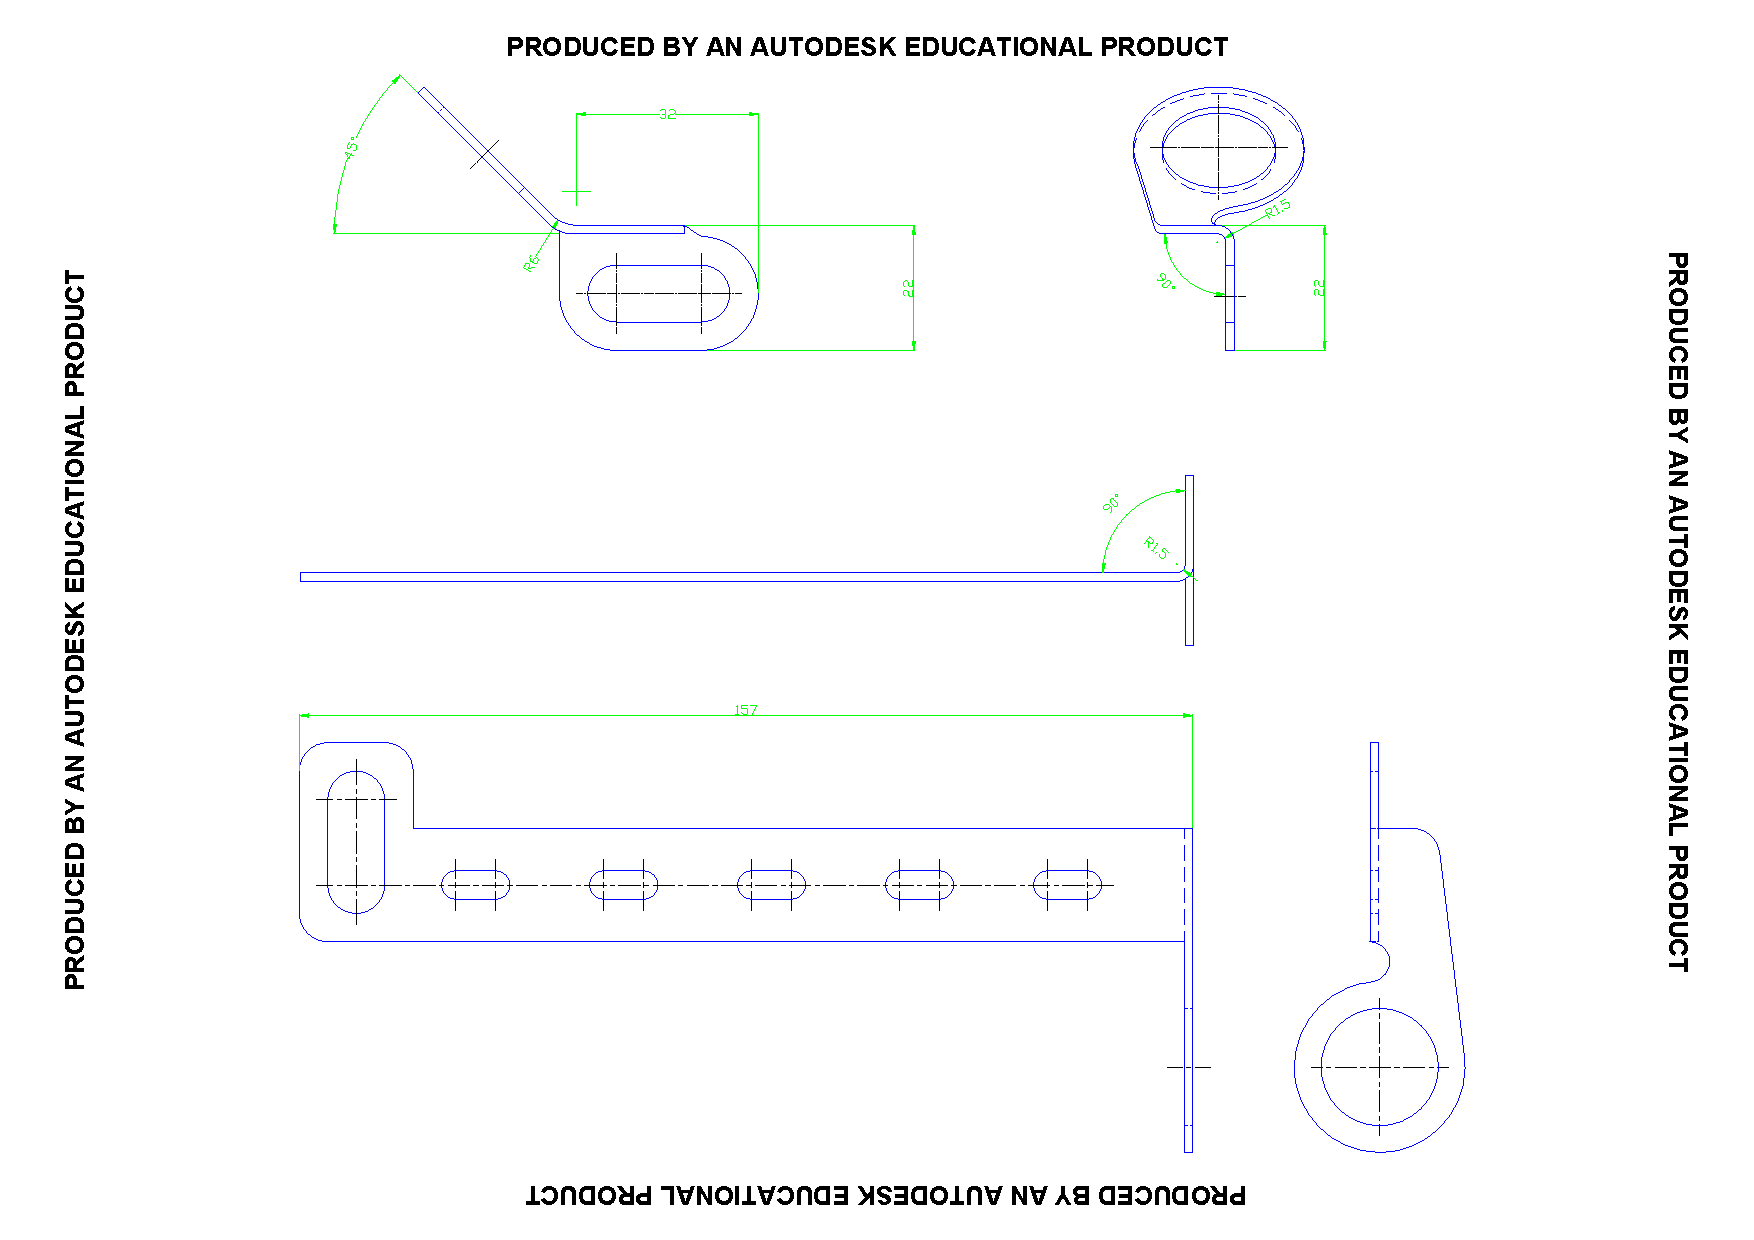
\includegraphics[width=7.5cm,trim = 2cm 1cm 2cm 1cm, clip]{pics/PIC007.pdf}
%		\caption{The upper and lower port side brackets for the radiator}
%		\label{fig:PIC007}
%	\end{center}
%\end{figure}
%\end{frame}

%\subsection{Cabin heating system}
%
%\begin{frame}\frametitle{Cabin heating system}
%\begin{figure}[ht!]
%	\begin{center}
%		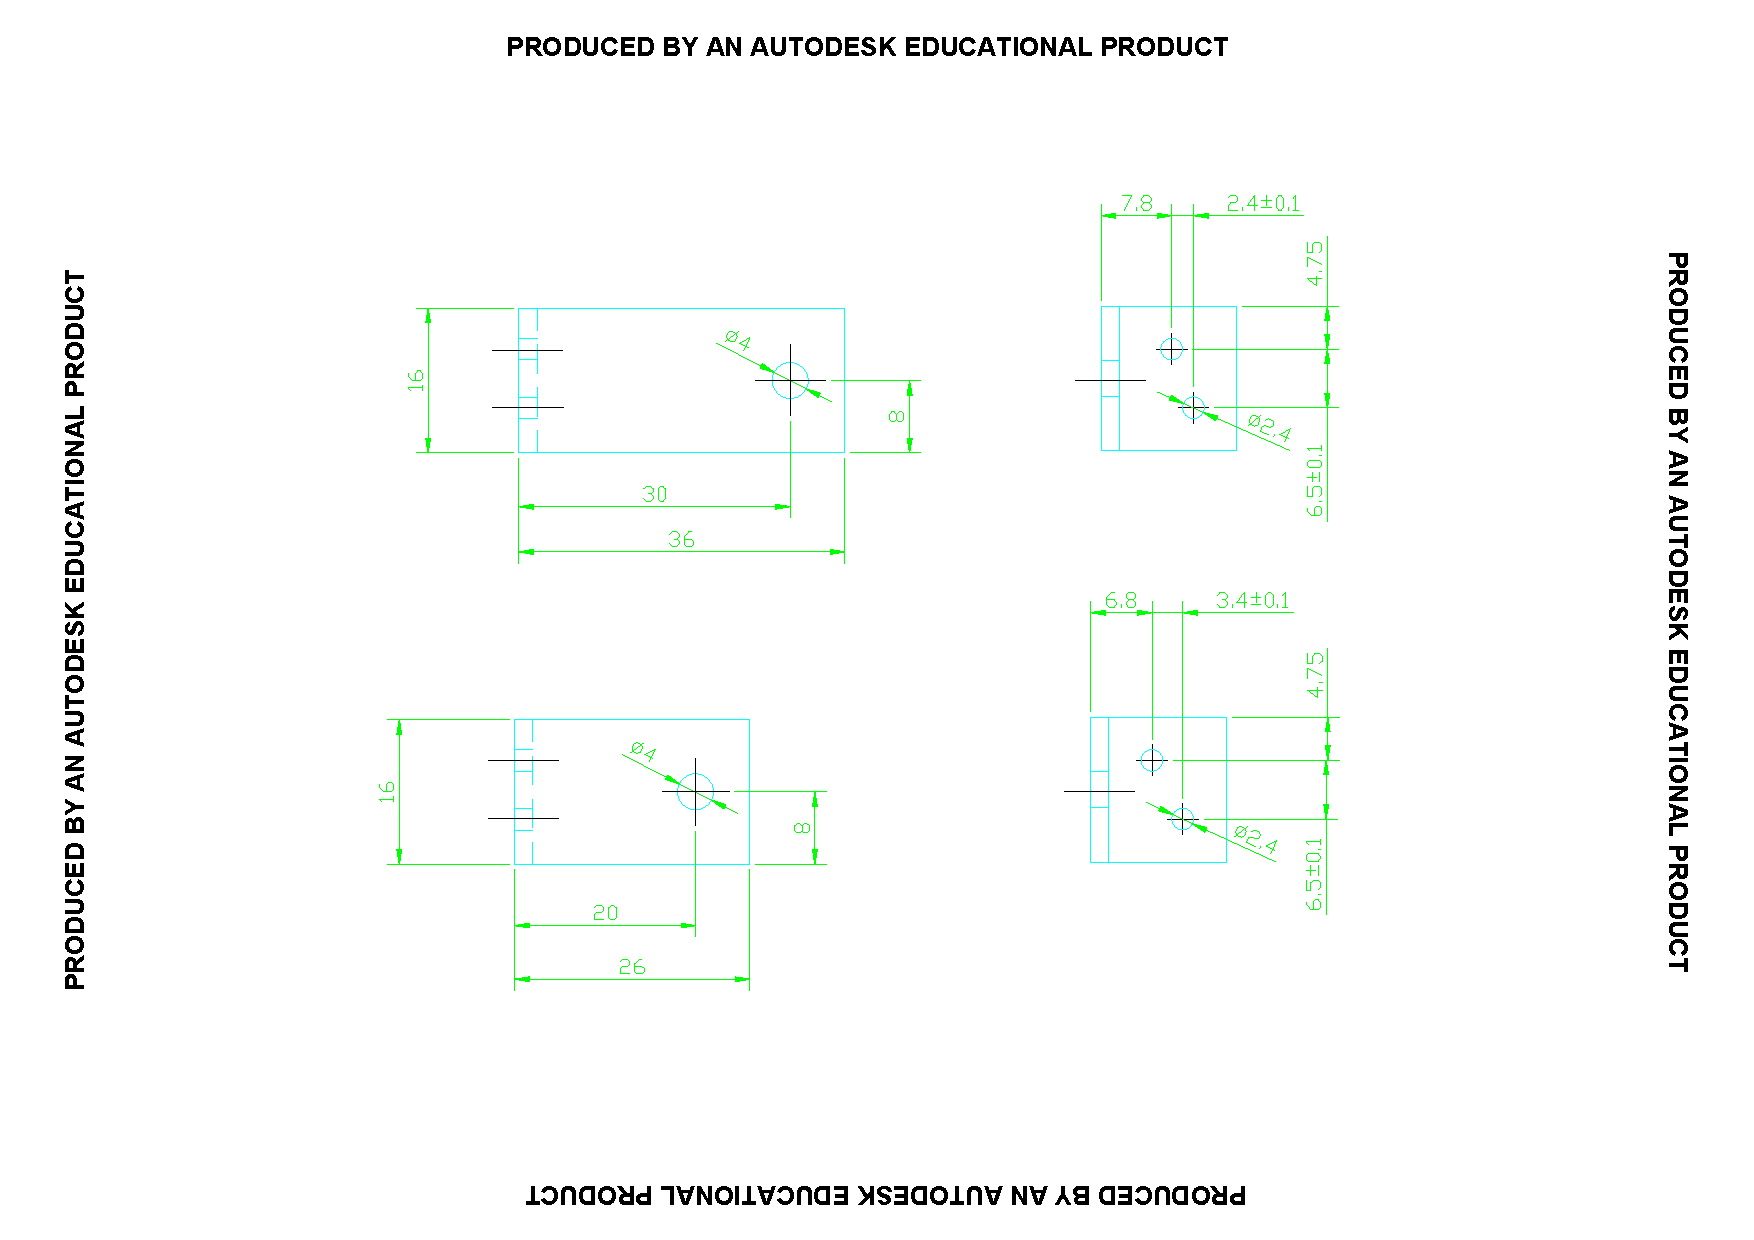
\includegraphics[width=7cm,trim = 6cm 4cm 6cm 3cm, clip]{pics/PIC009.pdf}
%		\caption{The L-brackets in the cabin heating system}
%		\label{fig:PIC009}
%	\end{center}
%\end{figure}
%\end{frame}

\subsection{Instrument panel - IPC}

\begin{frame}\frametitle{Instrument panel}
\begin{figure}[ht!]
	\begin{center}
		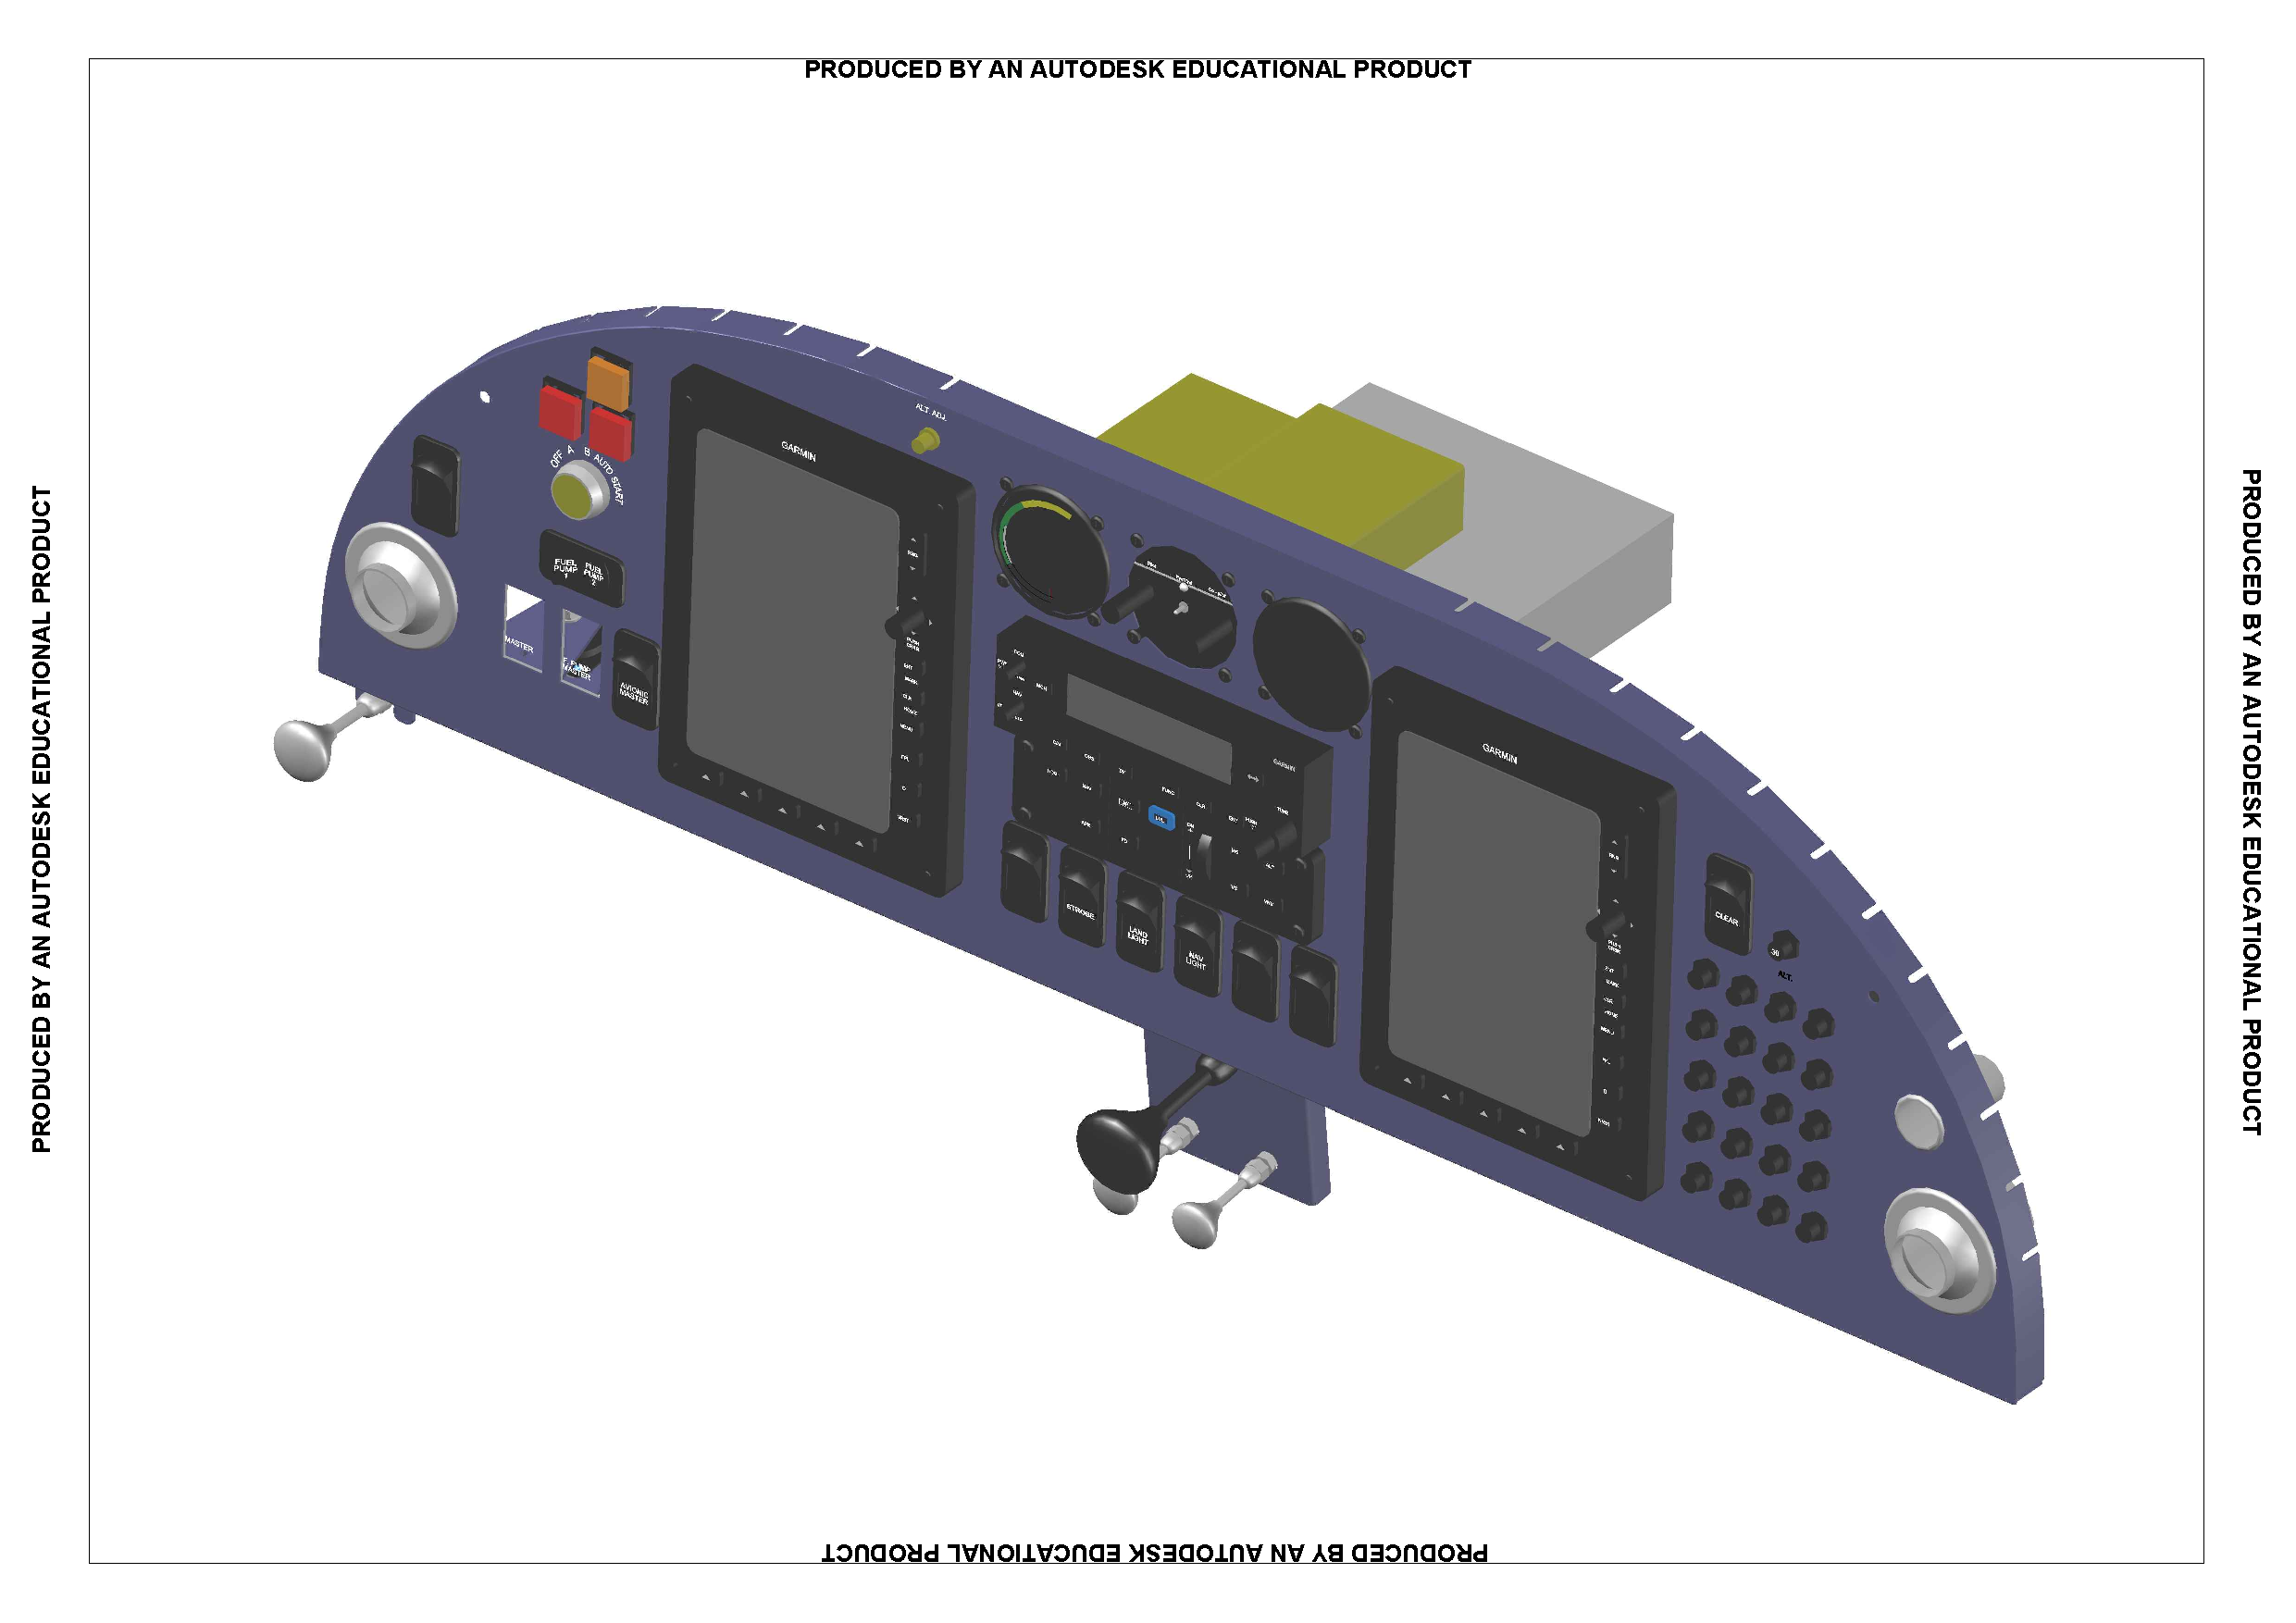
\includegraphics[width=8cm,trim = 4cm 4.cm 4cm 4.cm, clip]{pics/PIC030.pdf}
		\caption{The instrument panel}
		\label{fig:PIC030one}
	\end{center}
\end{figure}
\end{frame}

\begin{frame}\frametitle{Instrument panel}
\begin{figure}[ht!]
	\begin{center}
		\includegraphics<1>[width=10cm,trim = 2.8cm 2.8cm 2.8cm 2.8cm, clip]{pics/PIC034.pdf}
		\label{fig:PIC034}
		\includegraphics<2>[width=10cm,trim = 2cm 2cm 2cm 2cm, clip]{pics/PIC033.pdf}
		\label{fig:PIC033}
		\includegraphics<3>[width=10cm,trim = 2cm 2cm 2cm 2cm, clip]{pics/PIC032.pdf}
		\label{fig:PIC032}
		\includegraphics<4>[width=10cm,trim = 2cm 2cm 2cm 2cm, clip]{pics/PIC031.pdf}
		\label{fig:PIC031}
		\includegraphics<5>[width=10cm,trim = 2cm 2cm 2cm 2cm, clip]{pics/PIC030.pdf}
		\label{fig:PIC030}
	\end{center}
\end{figure}
\end{frame}

\begin{frame}\frametitle{Instrument panel}
\begin{figure}[ht!]
	\begin{center}
		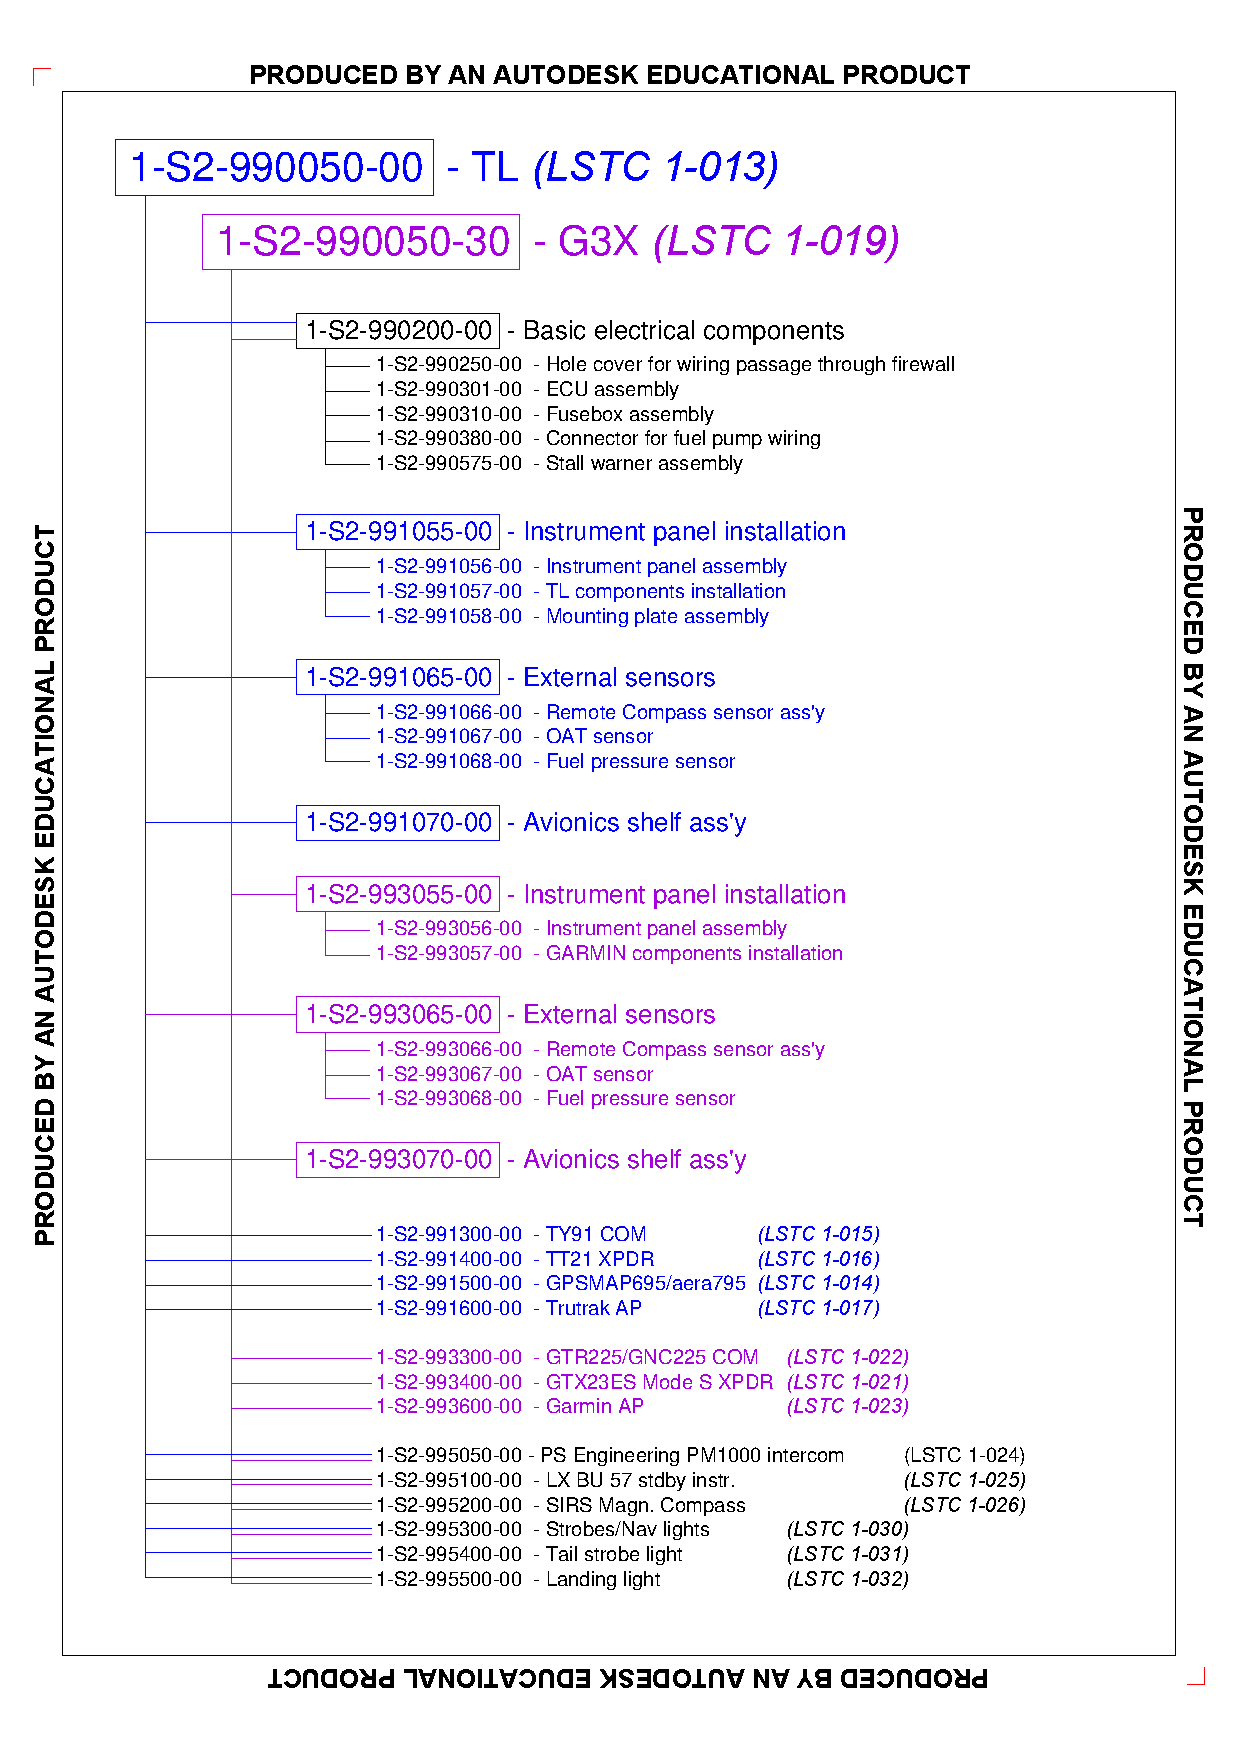
\includegraphics[width=4cm,trim = 1.9cm 2.4cm 1.9cm 2.4cm, clip]{pics/PIC015.pdf}
		\caption{The IPC structure for the electrical system}
		\label{fig:PIC015}
	\end{center}
\end{figure}
\end{frame}

\subsection{Instrument panel - IFR design}

\begin{frame}\frametitle{Instrument panel - IFR design}
\begin{figure}[ht!]
	\begin{center}
		\includegraphics[width=7.5cm]{pics/M108-IFR.jpg}
		\caption{The IPC structure for the electrical system}
		\label{fig:PIC015}
	\end{center}
\end{figure}
\end{frame}

%\subsection{Brake system}

%\begin{frame}\frametitle{Brake system}
%\begin{figure}[ht!]
%	\begin{center}
%		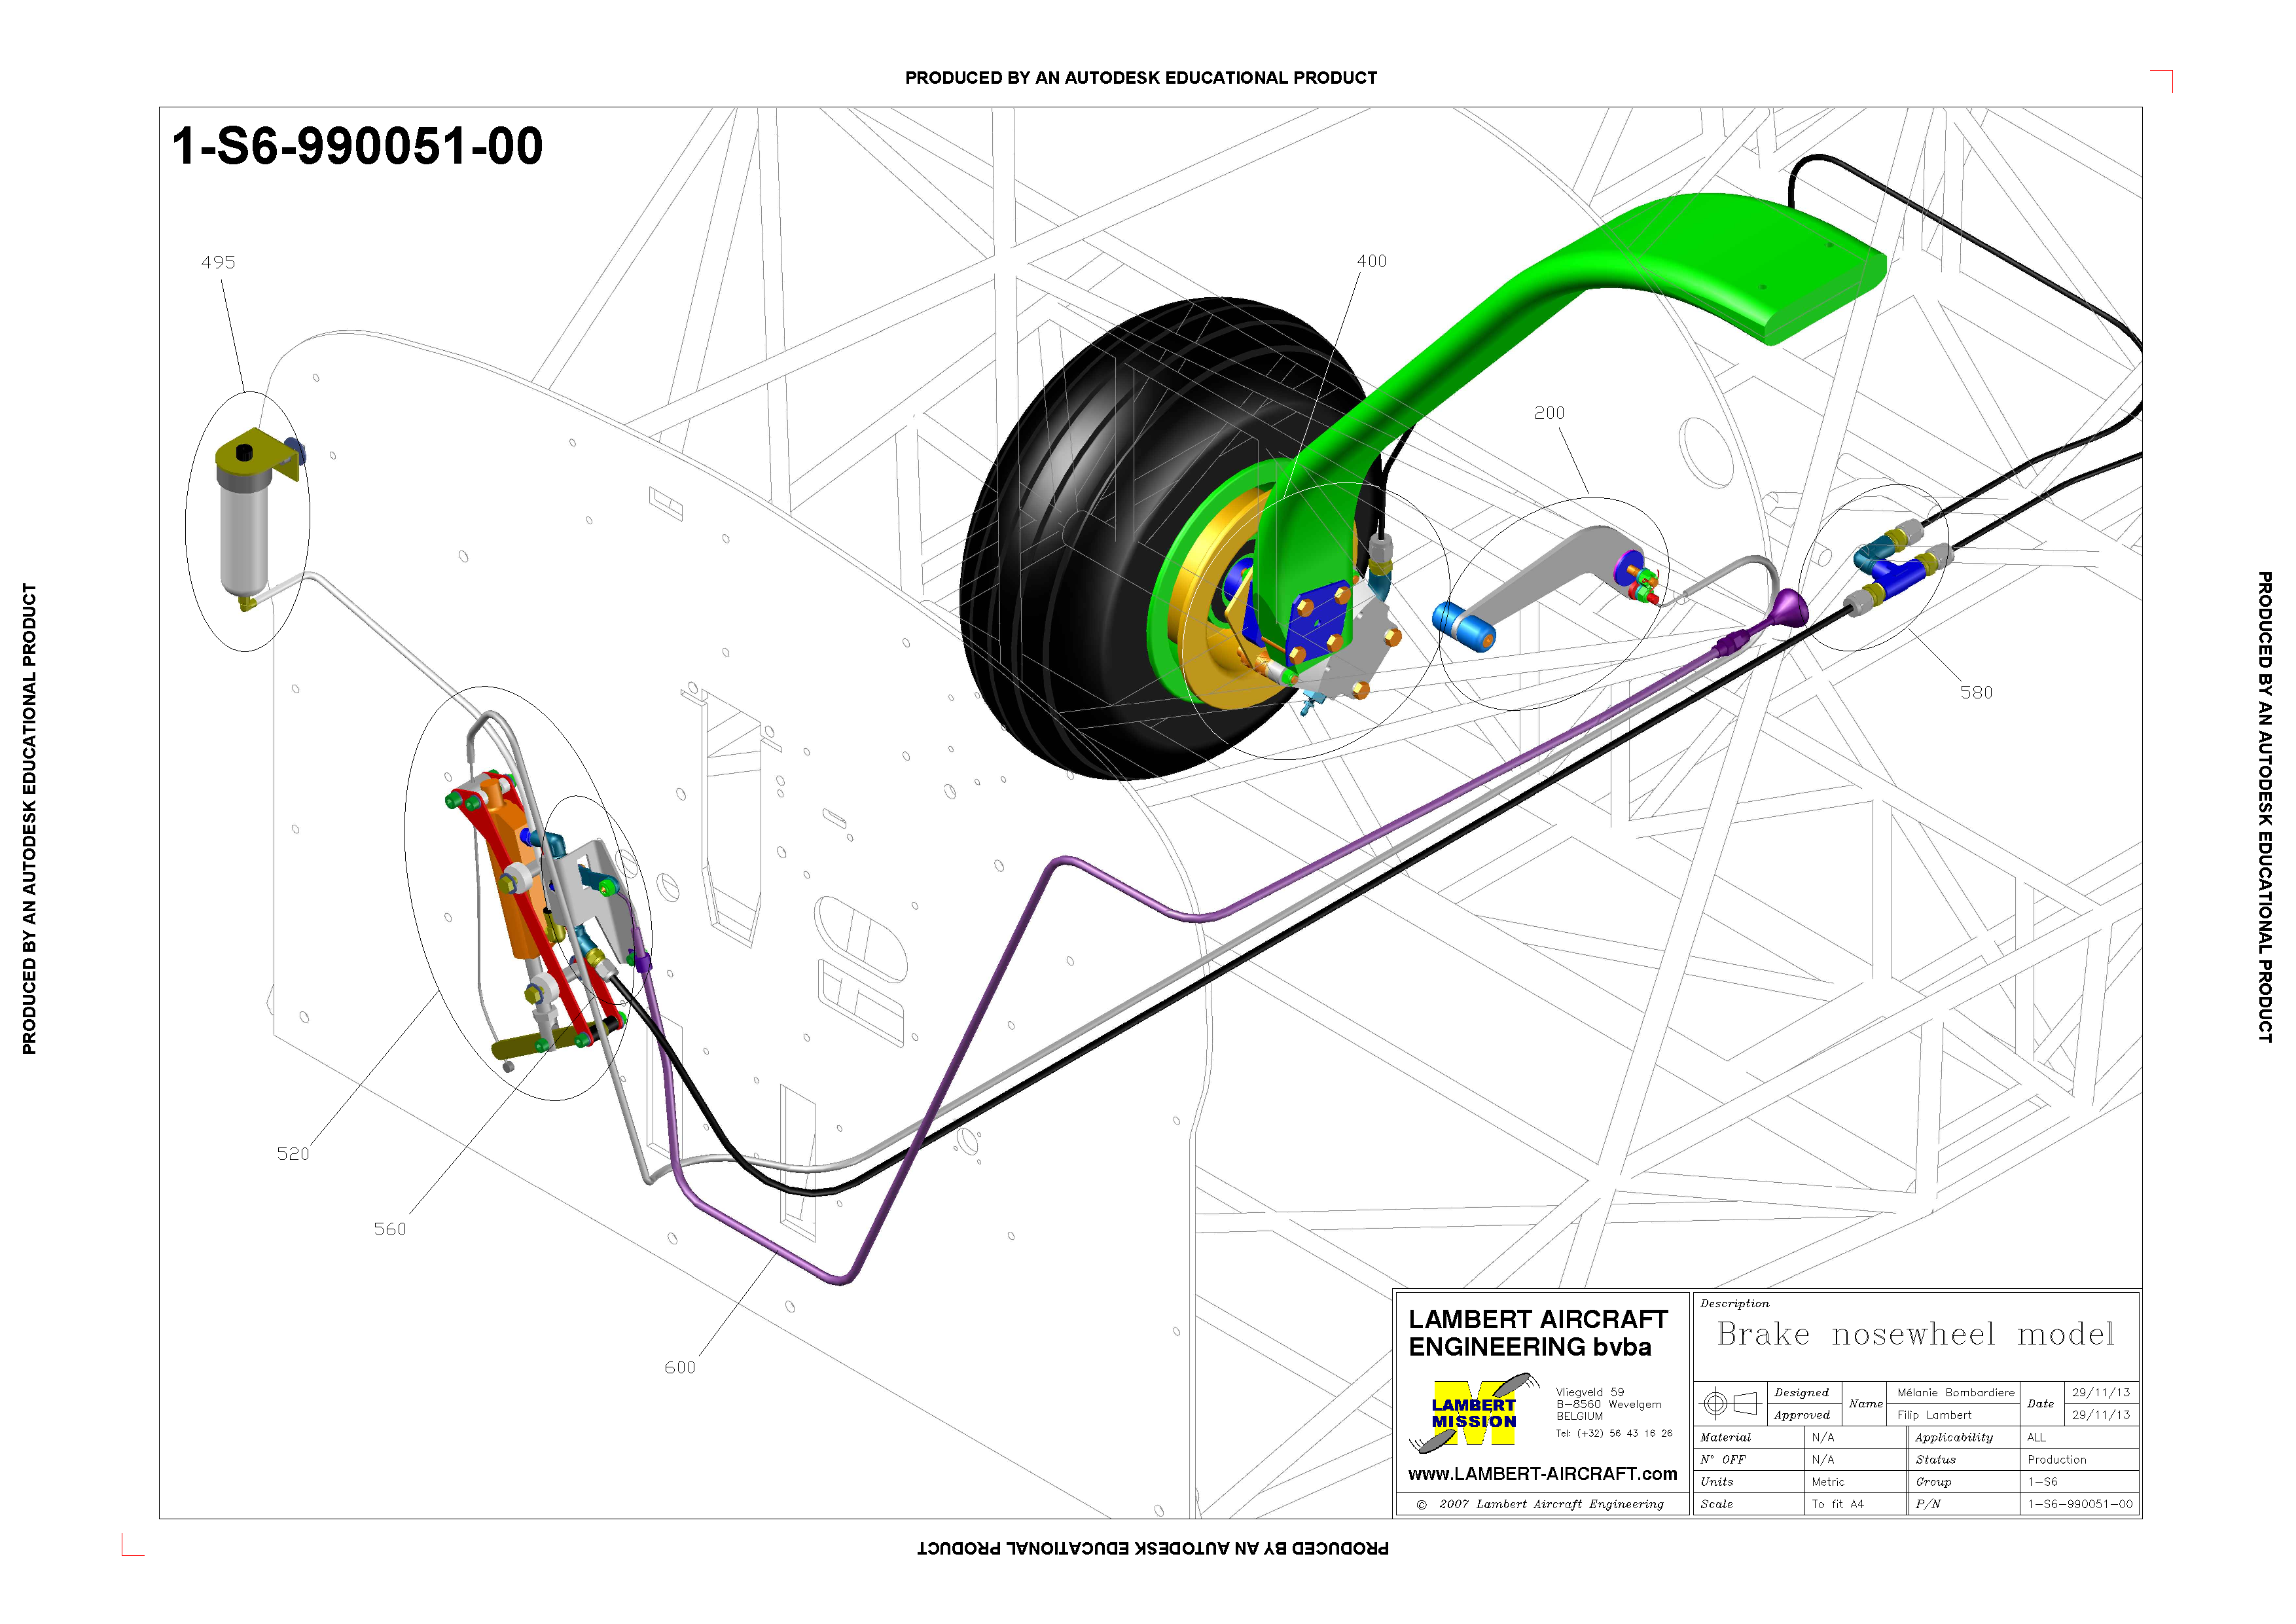
\includegraphics[width=10cm,trim = 1.5cm 2.5cm 1.5cm 2.5cm, clip]{pics/PIC019.pdf}
%		\label{fig:PIC019}
%	\end{center}
%\end{figure}
%\end{frame}

%\begin{frame}\frametitle{Brake system}
%\begin{figure}[ht!]
%	\begin{center}
%		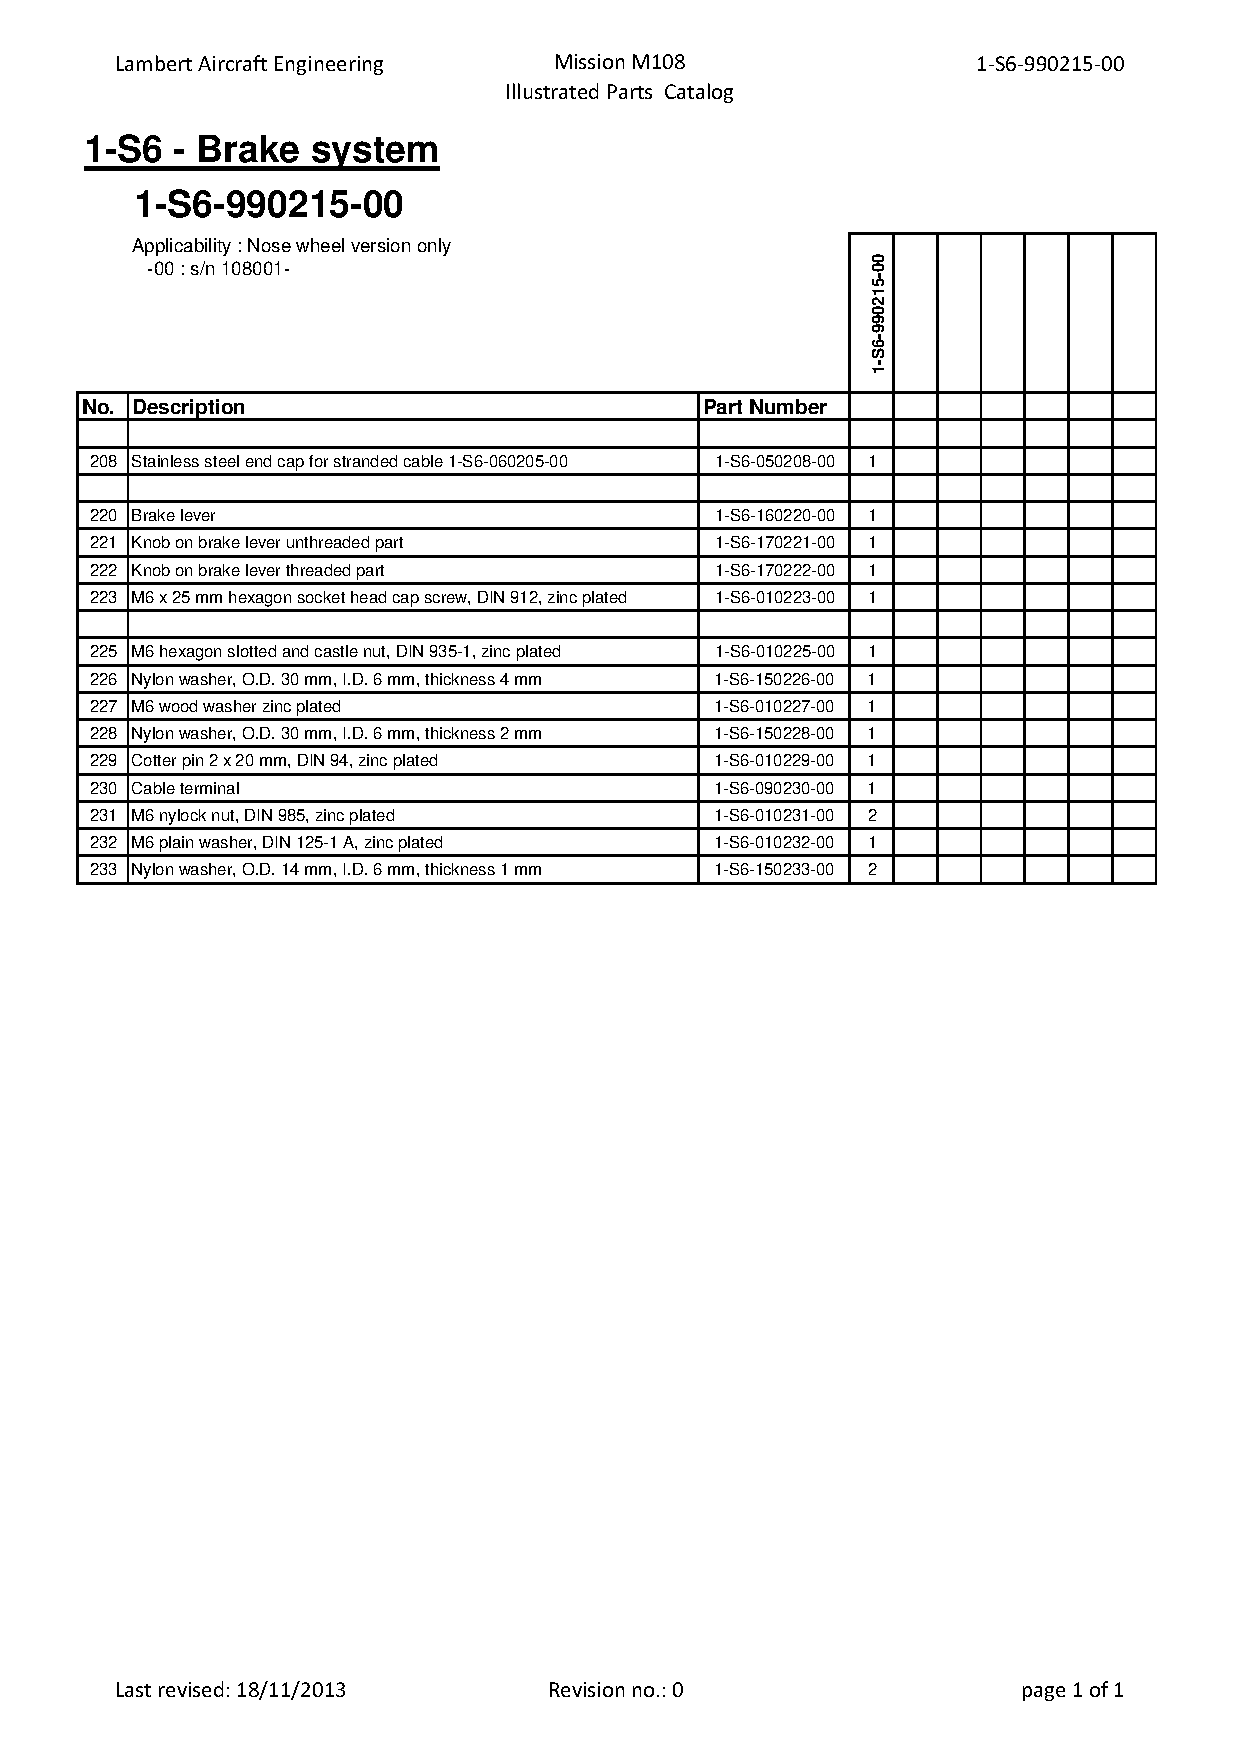
\includegraphics[width=10cm,trim = 1cm 8cm 1cm 2.25cm, clip]{pics/PIC011.pdf}
%		\label{fig:PIC011}
%	\end{center}
%\end{figure}
%\end{frame}

%LINK BETWEEN DATABASE AND IPC -- EXCEL SHEET
%We wanted something that blablabla... so we did blablabla

%\section{Database}
%\subsection{Database presentation}
%
%\begin{frame}\frametitle{Database}
%LAMS (Lambert Aircraft Management System)
%\begin{itemize}
%\item identifying parts in assemblies;
%\item stock control;
%\item cost calculations.
%\end{itemize}

%\end{frame}

%\subsection{Database structure}
%\begin{frame}\frametitle{Database structure}
%\begin{figure}[ht!]
%	\begin{center}
%		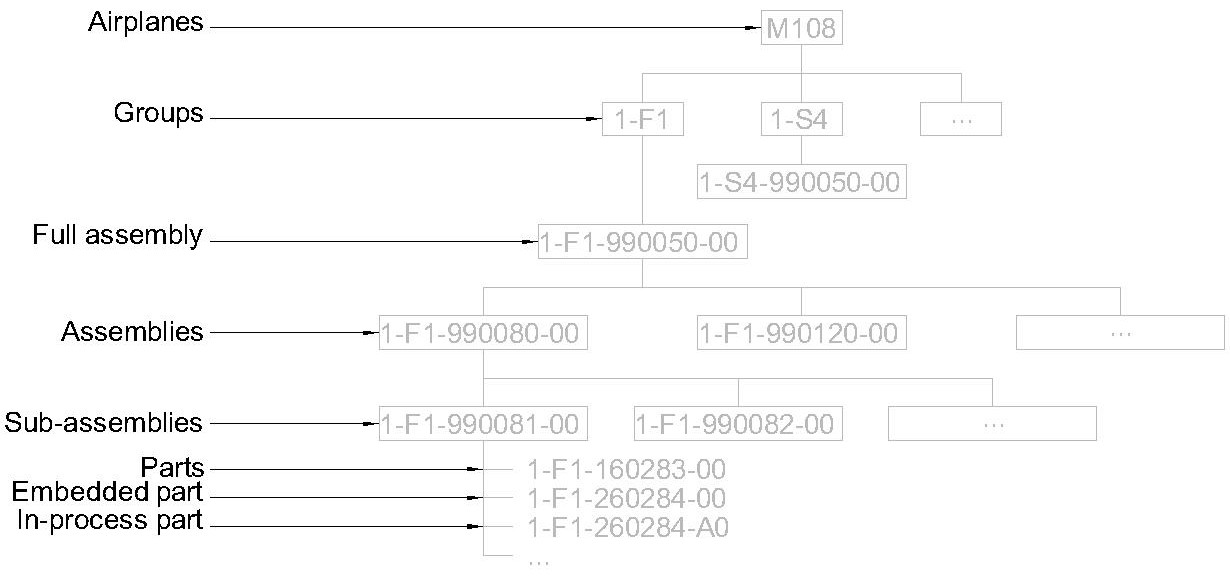
\includegraphics[width=11.5cm]{pics/PIC024.jpg}
%		\label{fig:PIC024}
%	\end{center}
%\end{figure}
%\end{frame}

%\subsection{Database test}
%\begin{frame}
%\begin{figure}[ht!]
%	\begin{center}
%		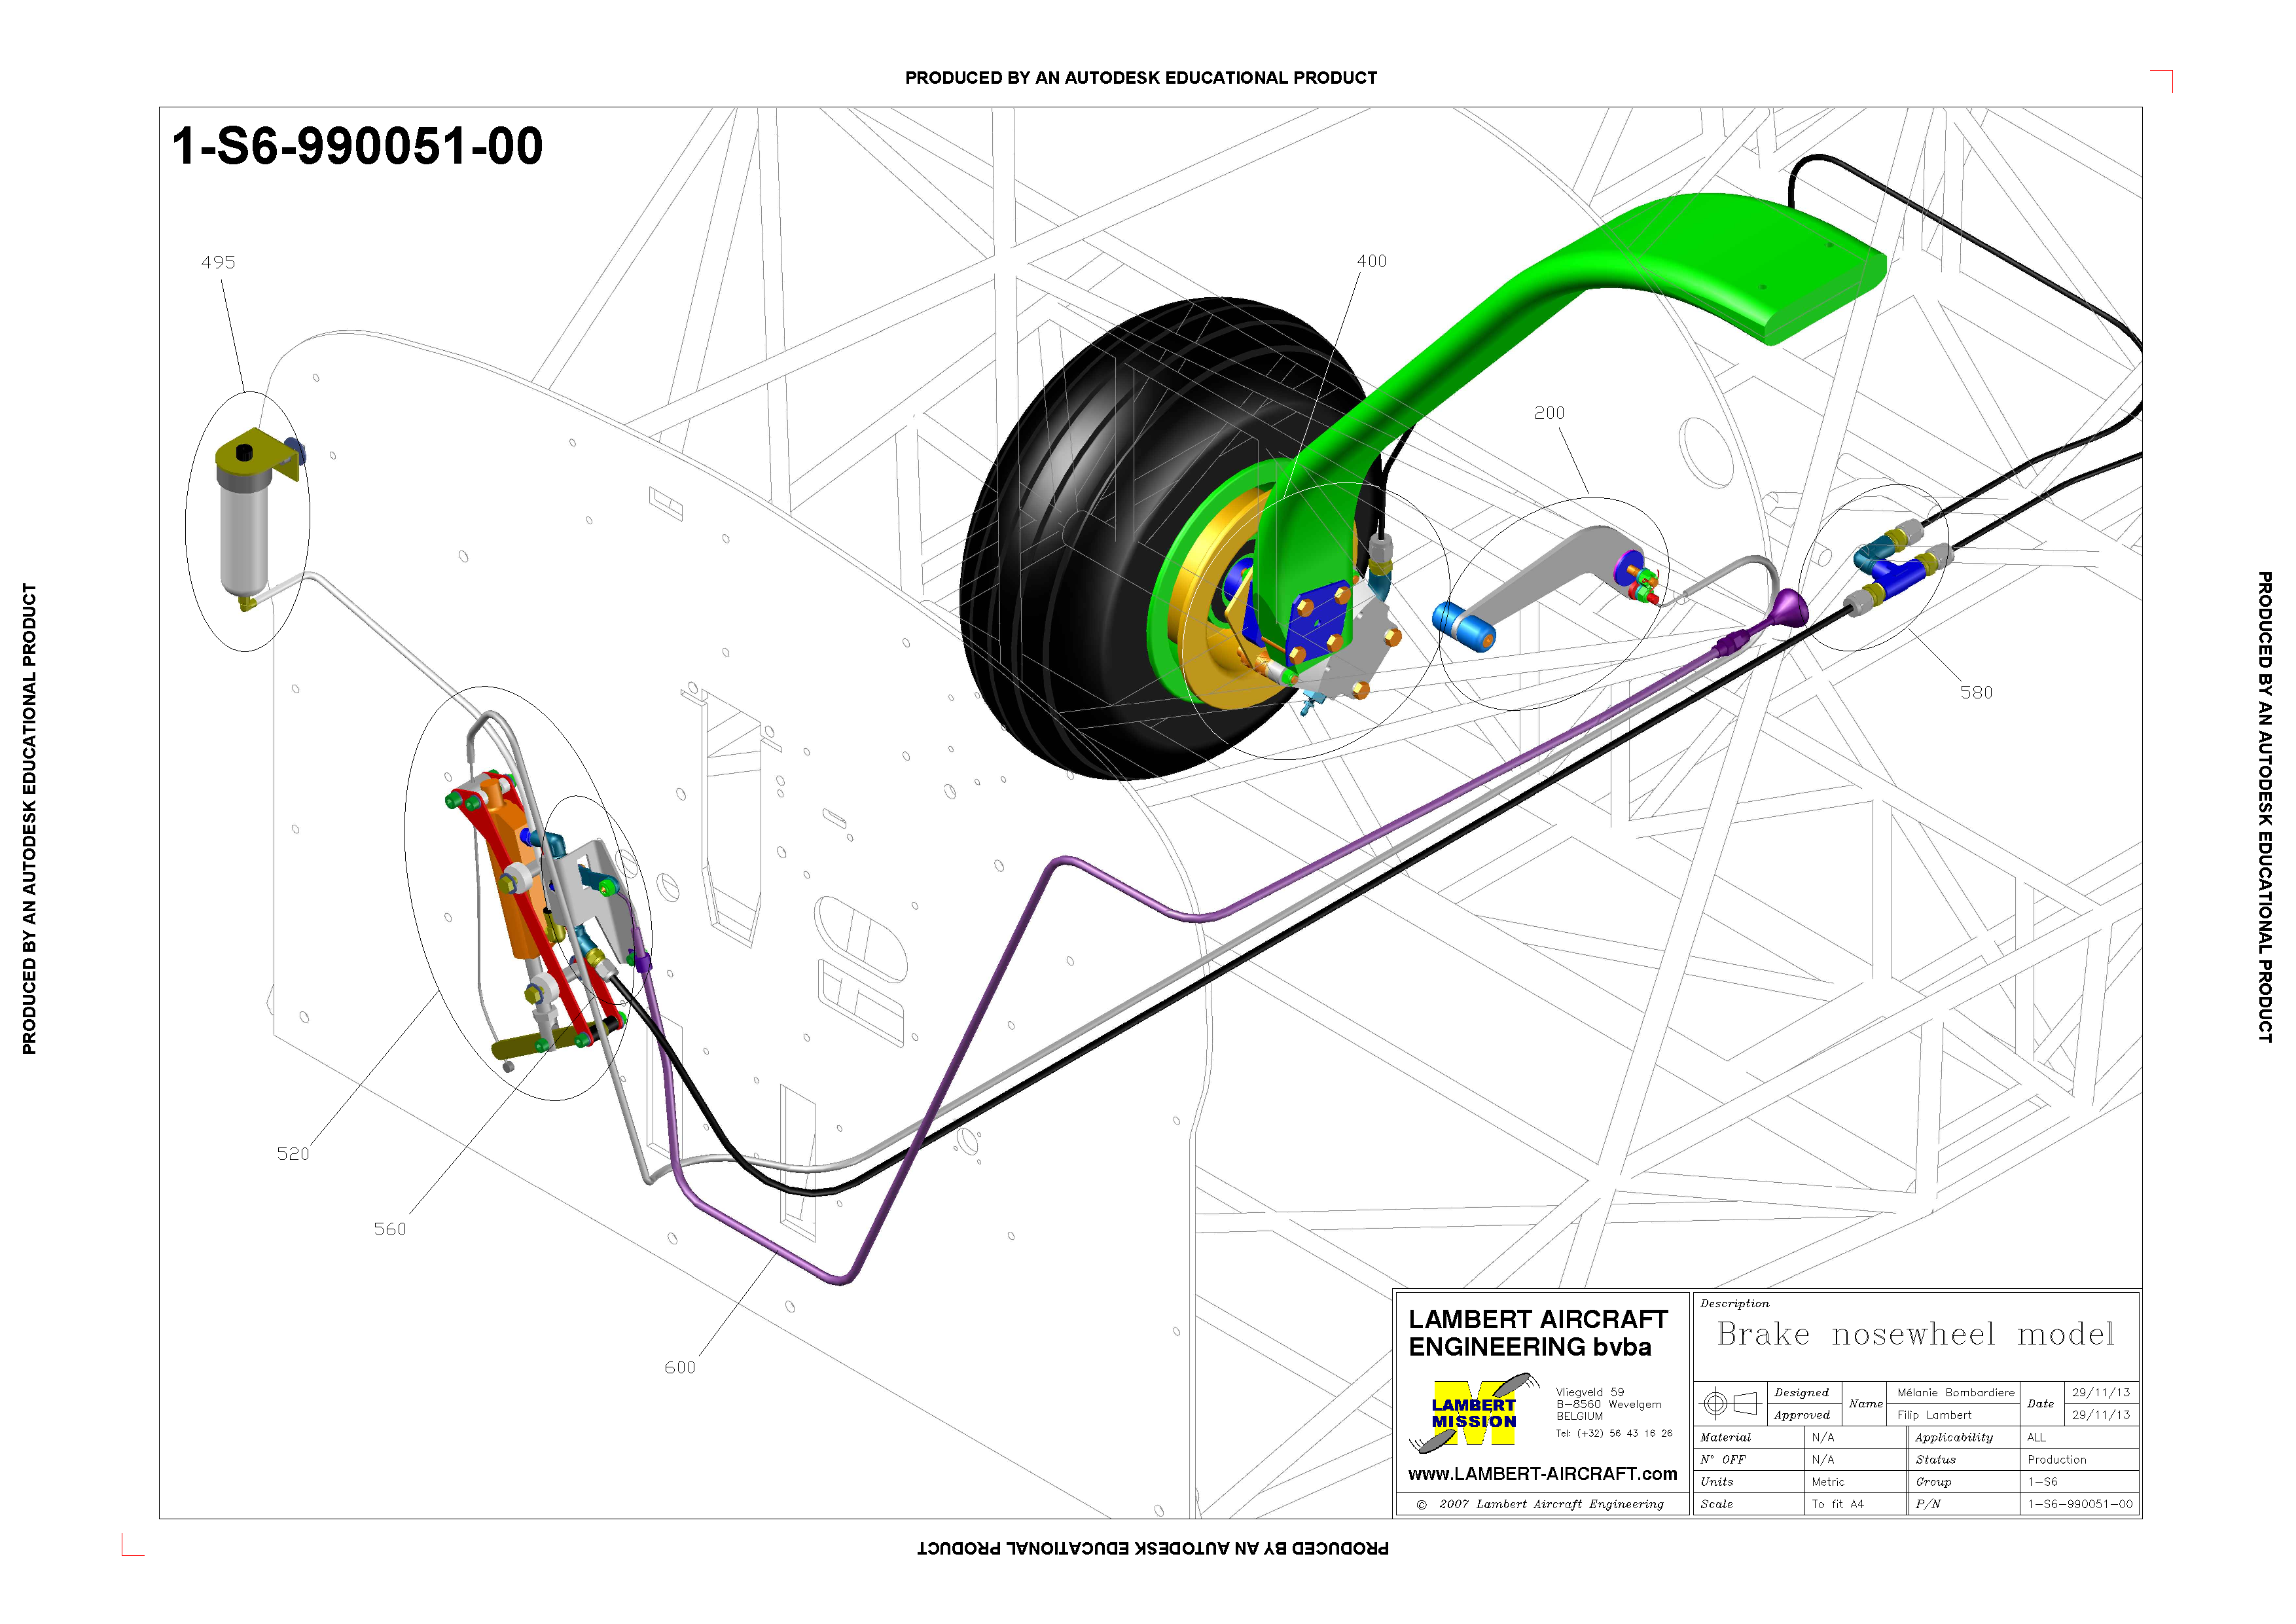
\includegraphics[width=10cm,trim = 1.5cm 2.5cm 1.5cm 2.5cm, clip]{pics/PIC019.pdf}
%		\label{fig:PIC019}
%	\end{center}
%\end{figure}
%\end{frame}

\section{Results}
\subsection{Contribution}

\begin{frame}\frametitle{Results -- Contribution}
\begin{itemize}
\item CAD and design work:
\begin{itemize}
\item Schematics and illustrations ;
\item Engine assembly: example of the radiator;
\item Cabin heating system: prevention and poka-yoke;
\item Illustrated Parts Catalog: combining 3D design and logic;
\item Pitot \& static systems: rethinking existing systems;
\item Brake installation: designing a new system.
\end{itemize}
\item Database.
\end{itemize}
\end{frame}

\subsection{Human experience}

\begin{frame}\frametitle{Results -- Human experience}
\begin{itemize}
\item Exchanging information;
\item Communication with the customer.
\end{itemize}
\end{frame}

\section{Conclusion}

\begin{frame}\frametitle{Conclusion}
\begin{itemize}
\item Objective of the internship;
\item Design team.
\end{itemize}
\end{frame}

\begin{frame}\frametitle{Conclusion}
\begin{itemize}
\item Willingness to leverage existing products \& tools;
\item Being able to take decisions quickly;
\item \textbf{Getting things done!}
\end{itemize}
\end{frame}

\end{document}
